\chapter{Aerodynamic Analysis}
\setlength{\parindent}{15pt}
\label{ch:aero_anal}

The aerodynamic analysis for horizontal flight only will be performed in this chapter, seeming that for vertical flight the airspeed will be low. The aircraft will need to fulfil a set of requirements which concern the aerodynamic properties of the aircraft. The most important aerodynamic property is the lift, since the aircraft will need to generate enough lift to be able to fly. The problem is that with lift comes drag. The challenge will be to design an aircraft which satisfies the requirements, while producing as little drag as possible.

The first section in this chapter is the approach, which is important to ensure that the process of designing goes well. The next section contains the assumptions made to ease the design process. The following section contains the actual analysis made for all the aerodynamic parts of the aircraft. Finally, once the analysis is done, the used methods are verified and validated. 

\section{Design Approach}

There are several aspects of the plane that need an aerodynamic analysis, each of these aspects will be designed to have the least amount of drag as possible. The problem that arises is that the design with the least drag probably will not coincide with the requirements or the constraints put up by other departments. This results in an iterative process which will ensure that the design with the least drag, and that complies with requirements and constraints, comes out best. To get an overview of the design process, \autoref{fig:flow:aerodynamics} shows the process followed in the form of a work flow diagram.

\begin{figure}[hbt]
    \centering
    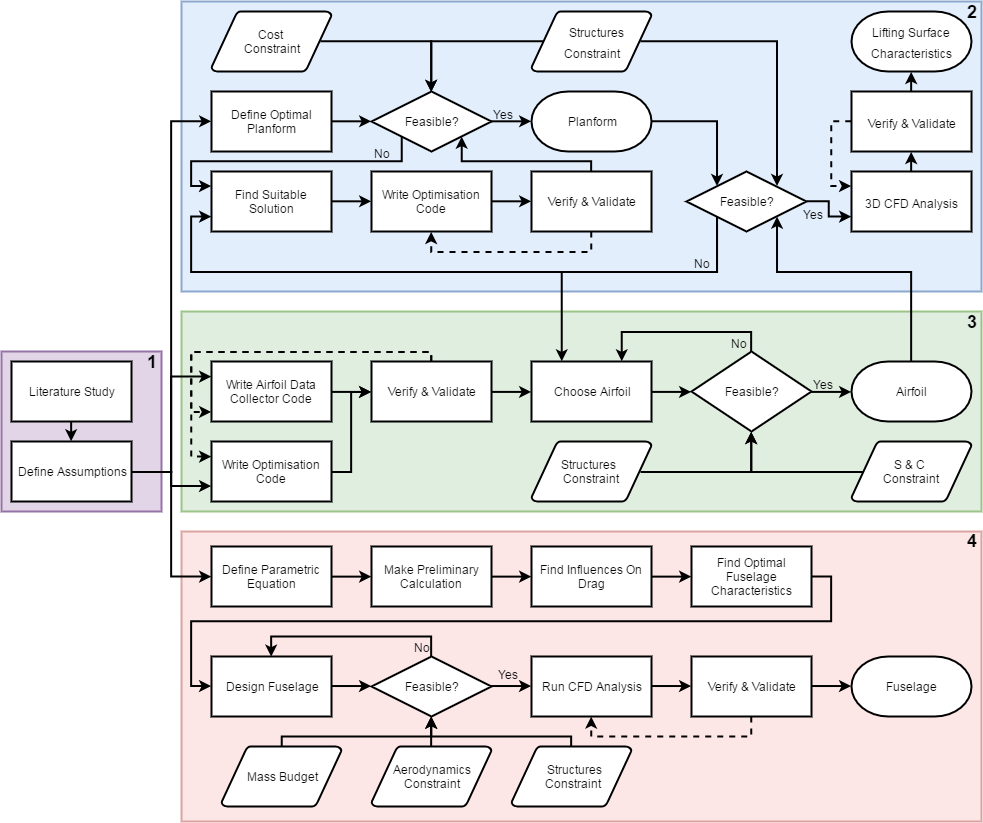
\includegraphics[scale=0.45]{Aerodynamics/Figures/AerodynamicWFD.png}
    \caption{Work Flow Diagram for the Aerodynamic Design Process}
    \label{fig:flow:aerodynamics}
\end{figure}

The work flow diagram shows four differently coloured regions. These are the separate processes that have been carried out, though not only four processes have taken place. The first region is the preparatory work needed to be done before the designing can start. The literature study will help with understanding how to perform the design, and the assumptions will be made to give an overview of how the design can be done. Once that is finished, it is possible to go to any of the other regions based on what needs to be designed.

The second region contains the work flow diagram for the sizing and shaping of both the wing and the tail. The processes for both these subsystems are very similar, hence they have the same work flow diagram. The first step of the process is to define the optimal planform, which would be the one with the least amount of induced drag. Once that is done, it needs to be checked if the planform is feasible with the constraints set by the structures department. If feasible, then the planform is done. If it is not feasible, then an alternate solution has to be determined. With the help of a Python code the optimal alternative can be found, and again checked to be feasible. Now, if it is not feasible, the iteration starts to find the correct planform.

The third region is the work flow diagram for the airfoil selection for both the wing and the tail. Before this process can start, code has to be written to collect all airfoil data and select the optimal airfoil. Verification and validation will check if the code used is correct. Once all the data is collected and the optimisation is made, the airfoil will be checked for feasibility, constrained by the structures department and the stability \& control department. If the airfoil turns out to be infeasible, a new airfoil optimisation will be run with new constraints to find the new best airfoil.

The fourth region is used for the design of the fuselage and the pylon. To start off the process, several parametric equations are selected which are used to make preliminary calculations. Once the calculations are done, it is possible to find the major influences of the fuselage shape on the drag. Knowing these influences, the optimal fuselage characteristics can be found, with which it is possible to design the fuselage. Once again, when the fuselage is designed, it needs to be checked for feasibility. This time the constraints come from the structures department, the aerodynamics department and the mass budget. If the design is feasible, a Computational Fluid Dynamics [CFD] analysis can be done to find more precise aerodynamic characteristics. The results of the CFD analysis are reflected against the parametric equations to check whether the CFD analysis has been implemented correctly.

\nomenclature[A]{CFD}{Computational Fluid Dynamics}

\section{Assumptions}

\begin{itemize}
    \item The flight condition is assumed to be at an altitude of 120 meters. This has been chosen because the majority of missions will not be flown at higher altitudes, so it will be optimised for a 120 meter altitude. When flying at a higher altitude, the aircraft will need to fly at a higher angle of attack to achieve enough lift, increasing the drag and decrease the overall performance.
    \item The increment in velocity due to the pusher propellers is assumed to be negligible, not affecting the wing aerodynamics. In reality the propellers will increase the speed over the wing and decrease the amount of detached airflow, which increases the lift over the wing.
    \item The lifting surfaces are assumed to be completely smooth. In reality there are imperfections and other aspects, e.g. attachments, which decrease lift and increase drag.
    \item The drag of the propellers and motors is neglected. In reality they produce drag, but due to a lack of resources it was not possible to analyse this.
    \item The upwash and downwash of the wing on the pylons is neglected. In reality this effect would create a destabilising positive pitching moment. Nevertheless, ignoring this is acceptable as the pylons are narrow and the resulting pitching moment will be orders of magnitude smaller than the one created by the wing and tail.
    \item It is assumed that for the CFD analysis the boundary layer is completely laminar. In reality, the boundary layer will transition to a turbulent flow, yet it is assumed that the transition point is near the aft of each geometry. The direct effect is a lower skin friction drag than in the case when the transition is not neglected. \cite[75]{anderson}, \cite[170]{fluidmech}.
    \item It is assumed that for the CFD analysis the turbulence model is laminar. Since most geometries of the UAV are smooth, slender, and have a small angle of attack, it is assumed that in reality the transition from a laminar to a turbulent flow would not occur.
\end{itemize}

\section{Analysis}

This section will contain the analysis of the various subsystems. The goal of the analysis is to find the optimal solution to the problems at hand by meeting the requirements given with the set of constraints set by other departments. The first subsystem to be analysed is the wing in \autoref{sec:aero_wing}. Next, the tail will be analysed in \autoref{sec:aero_tail}, and the fuselage is analysed in \autoref{sec:aero_fuse}. The last subsystem analysed is the power \& propulsion subsystem, though only the pylon will be analysed. This analysis can be seen in \autoref{sec:aero_pylo}.

\subsection{Wing}
\label{sec:aero_wing}

There are five things that need to be analysed for the wing. The first aspect to be analysed is the shape \& size of the wing, which gives the wing planform. Afterwards, the airfoil can be found which will give the wing the best aerodynamic properties. When that is done, a look will be taken into the high lift devices to see if they are necessary. Finally, with the basic wing shape designed, it is possible to analyse the wing in a 3D environment, to see if the aerodynamic characteristics are still satisfied. Finally, the winglets are the last aspect of the wing to be checked.

\subsection*{Shape \& Size}

\paragraph{Literature Study} For low speed aircraft, there is one major influence of the wing on the drag, namely the induced drag\footnote{\url{https://www.grc.nasa.gov/www/k-12/airplane/induced.html}, Accessed on 14-06-2017}. Seeming this UAV flies at low speeds (20-55 $\frac{m}{s}$), the induced drag will be the biggest source of drag of the wing. To minimise the drag, the lift distribution of the wing needs to be elliptical, which can be achieved by having an elliptical planform. This would be the optimum planform of the wing, as can be seen in \autoref{fig:flow:aerodynamics}. However, an elliptical wing is harder to manufacture due to its complex shape \cite{ellipticalmanu}. Due to this, an alternative has to be found, which still resembles an elliptical lift the best. This can be done by using several taper ratios or having a different airfoil at different spanwise locations. Due to the seeming complex manufacturing of different spanwise airfoils, the choice has been made to have several different tapers to resemble an elliptical lift distribution.

Another aspect of the planform which has been looked at is the sweep of the wing. Usually the front is swept to reduce mach bubbles being created on the wing, which reduces lift drastically and generates a lot of drag. But this effect occurs only at high speeds (M \textgreater 0.8) so it is not necessary for this UAV to have it. Having a swept wing will only have an adverse effect by reducing the chord wise speed over the wing, hence reducing lift. If the lift decreases, a bigger surface area will be needed which would only increase the drag.

Having a wing stall can have an adverse effect on the safety of the aircraft, it gets even worse if the tip stalls before the root. This is because this will create a moment on the aircraft, which will roll the aircraft uncontrollably. This rolling can cause the aircraft to plummet to the ground, especially when close to the ground during landing. To prevent the tip stalling before the root, the tips will have washout. This causes the wing tips to have a lower incidence angle with respect to the rest of the wing, making it have a lower angle of attack. Due to the lower angle of attack, the tips will stall later and hence prevent tip stalling.

\paragraph{Method} The sizing of the wing has been done by looking at the wing loading. The surface area needed to generate enough lift depends on various factors, see \autoref{eq:liftgenerate}.

\begin{equation}\label{eq:liftgenerate}
    S = \frac{2\cdot W}{C_{L}\cdot V^2\cdot \rho}
\end{equation}

Using air density at sea level and the stall speed of 20 $\frac{m}{s}$, it is possible to find the wing loading for different $C_{L}$ values. The best $C_{L}$, at a feasible wing loading, is 1.3. With this number the surface area of the planform is calculated to be 0.8 $m^2$.

Since the optimum solution (an elliptical planform) is not feasible, it is necessary to find the best alternative solution. With the choice to have several different taper ratios, it has been chosen to use two different taper ratios on the wing. This choice has been made because the wing has to be detachable for ground handling, so the location of the taper change will be where the wing is detachable. Having more than two tapers would implicate the manufacturing while improving the planform slightly. 

To find the best planform, a python code has been made. The code has been made in such a way that it would iterate through all variables directly or indirectly to find all possible combinations of planforms. The variables can be seen in \autoref{tab:dimensionswing}. Each planform generated has been compared to an elliptical planform, using the mean squared error of the differences of normalised chord lengths. This way the planform which resembles an ellipse the most could be chosen. To verify the planform for its elliptical lift, the program XFLR5 has been used, which can generate the lift of a 3D wing and show its distribution. The resulting lift distribution can be seen in \autoref{fig:wdist} in \autoref{sec:aero_vali}.

\paragraph{Results}

With the design process done, the planform of the wing is finalised. The result can be seen in \autoref{fig:wingplanform}. The dimensions of the planform are summarised in \autoref{tab:dimensionswing}.

\begin{figure}[H]
    \centering
    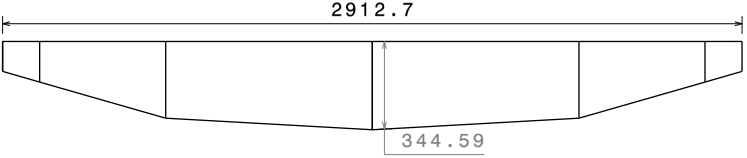
\includegraphics[scale=0.75]{Aerodynamics/Figures/wingplanform}
    \caption{Planform of the Wing, Dimensions in mm}
    \label{fig:wingplanform}
\end{figure}

\begin{table}[H]
    \centering
    \caption{Dimensions of the Wing}
    \label{tab:dimensionswing}
    \begin{tabular}{llll}\toprule
\bfseries    Variable     &\bfseries  Value &\bfseries Variable &\bfseries Value\\ \midrule
    $c_{t_w}$     & 118mm & $c_{r_w}$ & 348mm\\
    $b_w$ & 2920mm & $AR_w$ & 10. \\
    $\lambda_{tip}$ & 0.39 & $\lambda_{root}$ & 0.8 \\
    $l_{twist}$ & 146mm & $l_{taperchange}$ & 642mm \\
    Twist angle at tip & $5^{\circ}$ & &\\ \bottomrule
    \end{tabular}
\end{table}



\nomenclature[B]{$c_{t_{w}}$}{Tip chord of wing \nomunit{m}}
\nomenclature[B]{$c_{r_{w}}$}{Root chord of wing \nomunit{m}}
\nomenclature[B]{$b_w$}{Span of wing \nomunit{m}}
\nomenclature[B]{$AR_w$}{Aspect Ratio of wing \nomunit{-}}
\nomenclature[G]{$\lambda_{tip}$}{Taper ratio at tip of wing\nomunit{-}}
\nomenclature[G]{$\lambda_{root}$}{Taper ratio at root of wing\nomunit{-}}
\nomenclature[B]{$l_{twist}$}{Length of twist on wing (one side) \nomunit{m}}
\nomenclature[B]{$l_{taperchange}$}{Length where taper changes, as seen from the tip \nomunit{m}}
\nomenclature[B]{$C_L$}{Lift coefficient \nomunit{-}}

\subsection*{Airfoil}

\paragraph{Literature Study} It is possible to achieve lift by employing various methods, one being the use of airfoils. These produce lift while minimising their drag contribution. Therefore it possible to achieve high efficiency, which in turn depends on the airfoil geometry. Airfoils are classified into families, and depending on which family the airfoil belongs to, different parameters are used to describe the geometry. Airfoils within one family will show similar shape characteristics, which also distinguish them from the other families. Since the aerodynamic performance is directly influenced by the shape, every airfoil family will therefore have distinct aerodynamic characteristics. Thus the application of the airfoil serves as the starting point for airfoil selection, starting with the selection of the airfoil family.

The most common airfoil families are the NACA 4-, 5-, and 6-digit series. The geometries of these airfoils are defined by the maximum camber value and position, the maximum thickness, and the family-specific parametric equations. Since the Hybrid UAV must be able to transition from horizontal to vertical flight, it is essential that the airfoil is predictable at low velocities and high angles of attack ensuring a safe transition. Therefore, the airfoil chosen for the Hybrid UAV must demonstrate gentle stall behaviour, which is true only with the NACA 4-digit series \cite{naca_series}. For this series, the first digit indicates the maximum camber, the second specifies the position of the maximum camber, and the last two digits indicate the maximum thickness of the airfoil. All these values are shown as a percentage of the chord.

Apart from the general aerodynamic behaviour, the airfoil's lift and drag (or $C_{l}$ and $C_{d}$) relationship must also be considered since it dictates the efficiency. In the case of the Hybrid UAV, two ratios are of greatest importance, namely $\frac{C_{l}}{C_{d}}$ influences the maximum range, and $\frac{C_{l}^{1.5}}{C_{d}}$ influences the maximum endurance \cite{perf}. Since the Hybrid UAV will mostly fly in cruise condition, the aim is to maximise both of these ratios for the lift coefficient required at cruise velocity, effectively yielding the optimal airfoil.

\paragraph{Method} The selection of the airfoil was done in two steps. Firstly, a list of all possible NACA 4-digit series airfoils was generated, with parameters ranging from 0008 to 5530. These were then inspected for their maximum lift coefficient and all airfoils which had a $C_{l,max}$ lower than 1.3 (dictated by the stall velocity) were discarded. 

The second step consisted of calculating the $\frac{C_{l}}{C_{d}}$ and $\frac{C_{l}^{1.5}}{C_{d}}$ at a $C_{l}$ value of 0.56 ($C_{l,cruise}$) for the remaining airfoils. Next, the airfoil with the highest $\frac{C_{l}}{C_{d}}$ ratio, and the airfoil with the highest $\frac{C_{l}^{1.5}}{C_{d}}$ ratio was found, yielding two airfoils optimised either for maximum range, or maximum endurance.

\paragraph{Results} The result of the airfoil selection yielded only one airfoil, namely the NACA 4417. This means that this airfoil has the highest $\frac{C_{l}}{C_{d}}$ and $\frac{C_{l}^{1.5}}{C_{d}}$ at $C_{l,cruise}$, and therefore is optimal for both maximum range and endurance. Its geometry can be seen in \autoref{fig:4417geo}.

\begin{figure}[H]
    \centering
    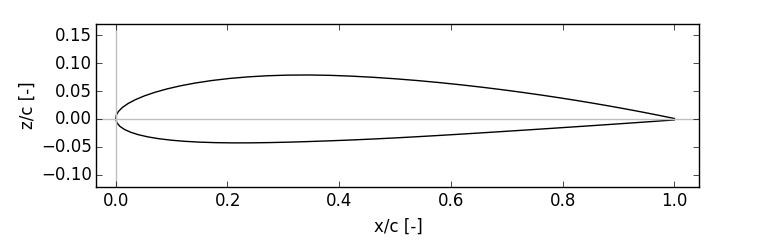
\includegraphics[scale=0.75]{Aerodynamics/Figures/4417geo}
    \caption{NACA 4417 Airfoil Geometry}
    \label{fig:4417geo}
\end{figure}
The aerodynamic characteristics of this airfoil are summarised in \autoref{tab:naca4417}. It should be noted that according to this analysis, the wing incidence angle is $1^{\circ}$ ensuring the highest efficiency in cruise flight.

\nomenclature[B]{$C_l$}{Lift coefficient of airfoil \nomunit{-}}
\nomenclature[B]{$C_{l,cruise}$}{Lift coefficient of airfoil during cruise \nomunit{-}}
\nomenclature[B]{$C_d$}{Drag coefficient of airfoil \nomunit{-}}


\begin{table}[H]
\centering
\caption{NACA 4417 Lift and Drag Characteristics}
\label{tab:naca4417}
\begin{tabular}{lcc}
\toprule
      & \textbf{Value} & \textbf{$\alpha$ {[}deg{]}} \\ \midrule
\textbf{$C_{l,max}$}    & 1.53  & 14                        \\ \hdashline
\textbf{$(C_{l}/C_{d})_{Cl,cruise}$} & 57.6  & 1                         \\ \hdashline
\textbf{$(C_{l}^{1.5}/C_{d})_{Cl,cruise}$} & 41.4  & 1                         \\ \bottomrule                                                                                
\end{tabular}
\end{table}

\subsection*{High Lift Devices}

\paragraph{Literature Study} High lift devices are necessary in aircraft to be able to fly at lower stall speeds, because the high lift devices increase the $C_{L}$ of the wing. This proves to be useful for large aircraft, so that the landing speed can be reduced significantly, ensuring a safer landing. However, the Hybrid UAV does not need to land horizontally, meaning that this is not a problem. High lift devices can still be implemented to be able to ensure a lower stall speed, but adding high lift devices brings forward more disadvantages than advantages. They will increase the overall cost of the aircraft due to extra material cost and manufacturing costs and it brings complexity in the wing which is unnecessary. More loads will be introduced, hence more structural integrity will be needed. These factors alone are the reason why the choice has been made not to use high lift devices.

\subsection*{3D Wing}

\paragraph{Literature Study} Determining the total lift and drag of the wing is essential when assessing the feasibility of the design. To do so, a three-dimensional analysis has to be performed which would mainly take into account the effect of the wingtip vortexes caused by the finite span. Two tools capable of such an analysis were found.

The first tool is XFLR5. It is an airfoil analysis tool also suitable for basic 3D wing analyses. For this software it was found that the horseshoe Vortex Lattice Method (VLM) is most fitting for the analysis since it allows non-flat wings to be analysed (the current wing has wing tip washout resulting in an out-of-plane geometry) \cite[26]{xflr}. In addition, XFLR5 has the option to include the effects of viscosity in the horseshoe VLM.

\nomenclature[A]{VLM}{Vortex Lattice Method}

The second tool is the SimScale Workbench, a CFD software. Starting with the meshing, it was found that the hex-dominant parametric meshing algorithm (included with the software) was most efficient and lead to faster convergence times \cite[9]{ansys}. Next, due to the very low Mach numbers, the fluid dynamics were selected to be incompressible. Furthermore, the turbulence model was selected to be laminar as explained previously in the assumption section. Finally it was found that smooth solvers are more efficient and therefore they were used as well \cite{iter}.

 It is expected that, with the use of the 3D analysis tools, the total lift will be smaller than $\frac{1}{2}\rho V^{2} S C_{l}$, the stall behaviour will be more gradual \cite[72]{ruijgrok}, and the total drag will be higher than $\frac{1}{2}\rho V^{2} S C_{d}$, where $C_{l}$ and $C_{d}$ are the airfoil lift coefficients.

\paragraph{Method} The 3D analysis was first carried out in XFLR5. The wing geometry was created within the tool and the surface was divided into panels. The panel distribution along the span is uniform (constant panel width), but along the chord a cosine distribution is used (panel size decreases towards the leading and trailing edge). Next, the viscous horseshoe vortex lattice method was chosen as the analysis definition. The analysis was ran with an initial velocity of 30 m/s and an angle of attack of $1^{\circ}$. The results were exported and analysed to find the total lift, drag, pitching moment, and lift distribution. Due to the iterative nature of the wing design, this process was repeated whenever necessary, and the results were updated. During the design iterations only XFLR5 was used for the 3D analysis since it could produce updated results within minutes, ensuring a smoother design process.

Once the wing design was fixed, the SimScale Workbench was used to determine the lift and drag with higher accuracy. First the wing geometry was imported into the program, and the corresponding surface and bounding-box meshes were created. The bounding box was made sufficiently large such that the boundary effects could be neglected. In addition, a second smaller mesh box was defined around the wing which consisted of a finer mesh. Next the inlet, outlet, and wall boundary conditions were set for the bounding box and wing surface. Finally, the simulation was started with an initial inlet velocity of 30 m/s. The analysis yielded the lift as well as the pressure and viscous drag.

\paragraph{Results} The first results of the XFLR5 analysis are seen in \autoref{tab:xflrwing}. As predicted, the total lift is lower than the one required to achieve flight at cruise conditions. Therefore an iteration was performed by increasing the $C_{l,cruise}$ and checking whether the previous airfoil remained the most efficient one. Since this was indeed the case, the wing incidence angle was changed to $2.5^{\circ}$, according to the 2D airfoil angle of attack corresponding to the new cruise lift coefficient. The results of the updated incidence angle are also seen in \autoref{tab:xflrwing}. The lift-drag polar for the wing can be seen in \autoref{fig:polar}.

\begin{table}[H]
\centering
\caption{Main Wing XFLR5 Results}
\label{tab:xflrwing}
\begin{tabular}{lccc}
\toprule
&\bfseries First Results &\bfseries Iterated Results & \\ \midrule
\textbf{$C_{L,cr}$}   & 0.444 & 0.622 & {[}-{]} \\\hdashline
\textbf{$L_{cr}$}    & 195.8 & 274.3 & {[}N{]} \\\hdashline
\textbf{$C_{D,cr}$}   & 0.015 & 0.02 & {[}-{]} \\\hdashline
\textbf{$D_{cr}$}    & 6.615 & 8.82 & {[}N{]} \\\hdashline
\textbf{$C_{M,ac}$} & -0.137  & -0.137  & {[}-{]} \\ \bottomrule
\end{tabular}
\end{table}

\begin{figure}[H]
    \centering
    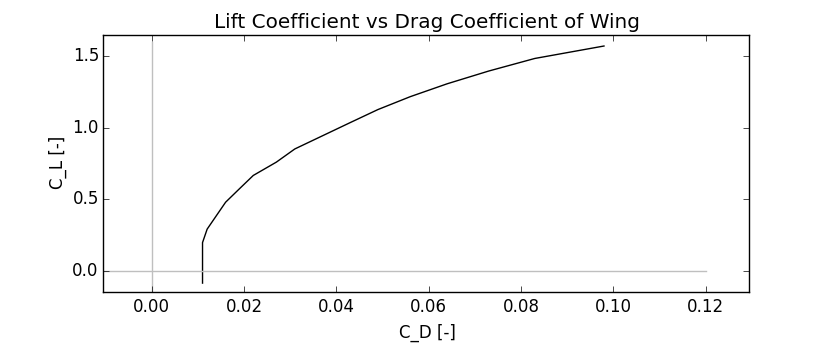
\includegraphics[width=0.8\textwidth]{Aerodynamics/Figures/wpol}
    \caption{Lift-drag Polar for the Wing}
    \label{fig:polar}
\end{figure}

The results of the SimScale Workbench CFD analysis with the updated wing incidence angle yielded a total lift of 173 N and a total drag of 6 N at cruise velocities. The validity of this result is discussed in \autoref{sub:vval}.

\subsection*{Wingtip Devices}

\paragraph{Literature Study} Wingtip devices such as winglets decrease the drag of a wing by reducing the magnitude of the tip vortices. This means the efficiency of the plane increases when using wingtips, although the factor it increases by is too low for further consideration\footnote{Prive Meeting with Mark Voskuijl, 15-06-2017}. Having the improved efficiency from the winglets does not overcome the disadvantages it brings with it. Having winglets increases the overall cost due to extra material for the surface and the internal structures (higher wing loading). Seeming the efficiency gained is not worth it, it has been decided not to use winglets.

\subsection{Tail}
\label{sec:aero_tail}

Only three aspects have to be analysed for the tail. The three aspects are similar to the wing, the shape, the airfoil and the 3D tail. The size of the tail will not be designed by the aerodynamics department because the surface area of the tail is of more value for the stability \& control department. The aspect to be analysed is the shape, which is done to design the planform of the tail (with the given surface area of the stability \& control department). The second aspect is the airfoil of the tail, which needs to comply with constraints set by the stability \& control department. The final aspect is the 3D tail, which is an aspect to be analysed because the 3D characteristics will differ compared to the 2D characteristics.

\subsection*{Shape}

\paragraph{Literature Study} There are two parts of the tail which need to be shaped and sized, namely the horizontal and the vertical tail. The empennage will be a T-tail type, chosen by the stability and control department. This means that the vertical tail will be closed in by the horizontal tail and the fuselage. Due to this, the vertical tail has been shaped in such a way that it would just fit between these two other parts of the aircraft. The horizontal tail however, has been shaped to minimise the drag. Just as for the wing, the minimal drag occurs when there is an elliptical lift distribution. This time, it is possible to achieve this with an elliptical planform due to three reasons. The first reason being that the loads on the horizontal tailplane are low, meaning the inner structure can be small and less complex. Furthermore, the size of the tailplane is much smaller than that of the wing, easing the manufacturing. The last reason is that the tailplane is not as complex as the wing. Due to these reasons the horizontal tailplane has been chosen to have an elliptical planform.

\paragraph{Method} The key to getting a elliptical lift distribution is to have the chord lengths follow the size of an ellipse, although the centre of the ellipse can be moved around. Keeping in mind that the elevators are most efficient if perpendicular to the flow, the horizontal centre line of the planform has been moved down to the three-quarters chord point. This way the elliptical lift distribution is kept while having a more effective controllability with the elevators. 

Having an elliptical lift distribution is not indicative of the root chord and span of the tailplane, so to size these dimensions reference aircraft have been used. The usual aspect ratio of a horizontal tailplane is between four and five\footnote{\url{http://nptel.ac.in/courses/101106035/035_Chapter\%206_L26_(04-10-2013).pdf}, Accessed on 20-6-2017}, for the vertical tail a taper ratio between 0.3-0.6 is common \cite{verticaltailtaper}. With these values, and the surface areas acquired from the stability \& control department, the final dimensions could be calculated for both the vertical and horizontal tailplane.


\paragraph{Results} With the shaping done, it is possible to find the dimensions of the tail surfaces. The dimensions of the tailplanes can be seen in \autoref{tab:taildimen}, the planforms of the horizontal tailplane and the vertical tailplane can be seen in \autoref{fig:htail} and \autoref{fig:vtail}, respectively.

\begin{table}[H]
    \centering
    \caption{Tail Dimensions}
    \label{tab:taildimen}
    \begin{tabular}{cc:cc}\toprule
    \multicolumn{2}{c}{\bfseries Horizontal Tail} & \multicolumn{2}{c}{\bfseries Vertical Tail} \\\midrule
    Parameter     &  Value & Parameter & Value\\ \midrule
    $c_{r_h}$     & 196mm & $c_{r_v}$ & 181mm\\ \hdashline
    $b_h$ & 694mm & $b_v$ & 220mm\\ \hdashline
    $AR_h$ & 4.5 & $AR_v$ & 3.35\\ \hdashline
    $\lambda_h$ & - & $\lambda_v$ & 0.45 \\\bottomrule
    \end{tabular}
\end{table}

\begin{figure}[H]
    \centering
    \begin{minipage}{0.45\textwidth}
        \centering
        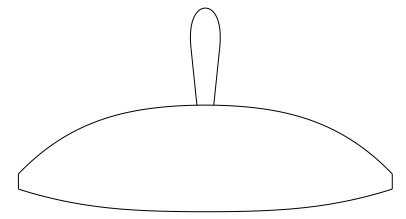
\includegraphics[width=0.9\textwidth]{Aerodynamics/Figures/htail} % first figure itself
        \caption{Top View of the Horizontal Tailplane, On Top Of The Vertical Tailplane}
        \label{fig:vtail}
    \end{minipage}\hfill
    \begin{minipage}{0.45\textwidth}
        \centering
        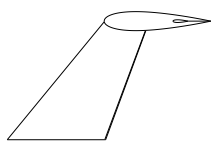
\includegraphics[width=0.9\textwidth]{Aerodynamics/Figures/vtail} % second figure itself
        \caption{Side View of the Vertical Tailplane}
        \label{fig:htail}
    \end{minipage}
\end{figure}

\nomenclature[B]{$c_{r_h}$}{Root chord of horizontal tail \nomunit{m}}
\nomenclature[B]{$c_{r_v}$}{Root chord of vertical tail \nomunit{m}}
\nomenclature[B]{$b_h$}{Span of horizontal tail \nomunit{m}}
\nomenclature[B]{$b_v$}{Span of vertical tail \nomunit{m}}
\nomenclature[B]{$AR_h$}{Aspect ratio of horizontal tail \nomunit{-}}
\nomenclature[B]{$AR_v$}{Aspect ratio of vertical tail \nomunit{-}}
\nomenclature[G]{$\lambda_v$}{Taper ratio of vertical tail \nomunit{-}}
\nomenclature[G]{$\lambda_h$}{Taper ratio of horizontal tail \nomunit{-}}






\subsection*{Airfoil}

\paragraph{Literature Study} The horizontal tail must stall later than the main wing to ensure stability, therefore the corresponding airfoil must have a larger stall angle than the one chosen for the main wing. Although the function of the horizontal plane is different from the main wing, the 4-digit NACA series is chosen here again as the starting point. This, again, is due to the predictable stall characteristics. In addition, this family is also common amongst tail airfoils \cite[23]{airtail}. Nevertheless, the main difference between the wing and the tail is that the tail usually uses a symmetrical airfoil since it must provide positive and negative lift. 

The required $C_{l_{h}}$ at cruise conditions (dictated by the stability \& control department) must also be kept in mind when selecting the airfoil, such that the tail will produce as little drag as possible during cruise, while keeping the UAV stable. Apart from the airfoil itself, the tail cruise lift coefficient can be changed by the horizontal plane incidence angle, yet the aim is to minimise this angle too.

\nomenclature[B]{$C_{l_{h}}$}{Airfoil lift coefficient of horizontal tail \nomunit{-}}

The vertical tail must produce the least amount of drag, therefore an appropriate airfoil must be chosen. The 4-digit NACA series is chosen for the vertical tail as well since, again, it is commonly used on tails. The only constraint on the vertical tail airfoil is the minimum thickness (dictated by the structures department), which in turn also depends on the vertical plane planform.

\paragraph{Method} The optimal horizontal tail airfoil was found by inspecting symmetrical NACA airfoils ranging from 0008 to 0029 for both the $C_{l_{h}}$ required at cruise conditions and the stall angle. It was decided that the stall angle should be about $4^{\circ}$ greater than the stall angle of the main wing. Out of all possibilities, the airfoil with the lowest thickness was chosen.

The optimal vertical tail airfoil was found by calculating the thickness of the vertical tailplane and comparing it to the structures department's requirement. The airfoil with the lowest sufficient thickness was chosen.

\paragraph{Results} The horizontal tailplane airfoil with the lowest thickness that satisfied the lift and stall requirements was the NACA 0018. The aerodynamic characteristics are summarised in \autoref{tab:naca0018}.

\begin{table}[H]
\centering
\caption{NACA 0018 Aerodynamic Characteristics}
\label{tab:naca0018}
\begin{tabular}{lcc}
\toprule
\textbf{$C_{l,cruise}$}  & 0.18 & [-] \\ \hdashline
\textbf{$C_{l,max}$}     & 1.24 & [-] \\ \hdashline
\textbf{$C_{d,cruise}$}  & 0.009 & [-] \\ \hdashline
\textbf{$\alpha_{stall}$} & 17.1 & [deg] \\ \bottomrule
\end{tabular}
\end{table}

The vertical tailplane airfoil with the lowest thickness that satisfied the Structures department's requirement was the NACA 0012. The zero lift drag coefficient ($C_{d_{0,v}}$) is 0.007.

\nomenclature[B]{$C_{l,max}$}{Airfoil maximum lift coefficient \nomunit{-}}
\nomenclature[B]{$C_{d,cruise}$}{Airfoil drag coefficient at cruise \nomunit{-}}
\nomenclature[G]{$\alpha_{stall}$}{Airfoil stall angle \nomunit{deg}}
\nomenclature[B]{$C_{d_{0,v}}$}{Airfoil zero-lift drag coefficient of vertical tail \nomunit{-}}

\subsection*{3D Tail}

\paragraph{Literature Study} The knowledge gained from the 3D Wing literature study is directly applicable to the 3D tail analysis. Again, it is expected that the 3D total lift will be smaller than the estimated 2D lift, and the 3D drag will be larger than the estimated 2D drag.

\paragraph{Method} The horizontal and vertical tailplane 3D analyses were first carried out in XFLR5 in the same manner as the main wing. The only difference is the angle of attack, which was now set to $0^{\circ}$ for both the horizontal and vertical plane. Hence, the horizontal plane has a incidence angle of $0^{\circ}$ as dictated by the stability \& control department.

Once the tail design was fixed, the SimScale Workbench was used again to determine the lift and drag with higher accuracy. This analysis was also carried out in the same manner as the main wing.

\paragraph{Results} The results of the XFLR5 tail analysis are seen in \autoref{tab:xflrhtail}. As predicted, the 3D lift coefficient of the horizontal tailplane is lower than the one required at cruise conditions. Therefore an iteration was performed by increasing the incidence angle of the horizontal plane to $2.6^{\circ}$. The iterated results are also shown in \autoref{tab:xflrhtail}.

\begin{table}[H]
\centering
\caption{XFLR5 Tail Results}
\label{tab:xflrhtail}
\begin{tabular}{lcccc}
\toprule
 & \textbf{Horizontal} & \textbf{Iterated Horizontal} & \textbf{Vertical} & \\ \midrule
\textbf{$C_{L,h}$}   & 0.118 & 0.181 & 0 & {[}-{]} \\ \hdashline
\textbf{$L_{h,cr}$}    & 6.96 & 10.68 & 0 & {[}N{]} \\ \hdashline
\textbf{$C_{D,h}$}   & 0.0015 & 0.0016 & 0.0003 & {[}-{]} \\ \hdashline
\textbf{$D_{h,cr}$}    & 0.65 & 0.71 & 0.128 & {[}N{]} \\ \bottomrule
\end{tabular}
\end{table} 

\nomenclature[B]{$C_{L,h}$}{Horizontal tail lift coefficient \nomunit{-}}
\nomenclature[B]{$L_{h,cr}$}{Horizontal tail lift at cruise \nomunit{N}}
\nomenclature[B]{$C_{D,h}$}{Horizontal tail drag coefficient \nomunit{-}}
\nomenclature[B]{$D_{h,cr}$}{Horizontal tail drag at cruise \nomunit{N}}

The results of the SimScale Workbench indicate a lift of 12.57 N and a drag of 1.11 N for the combined vertical and horizontal planes. The validity of these results is discussed in \autoref{sub:vval}.

\subsection{Fuselage}
\label{sec:aero_fuse}

\paragraph{Literature Study} From the point of view of the aerodynamics, the fuselage shape must be designed such that it produces the least amount of drag as possible during cruise flight. Based on the Roskam parametric equations for the fuselage drag, the two independent variables directly influencing the drag are the maximal frontal area and the length of the fuselage \cite[44]{roskam}.

Parametric equations serve as a starting point for the optimisation of the fuselage shape and provide an estimate on the drag, yet to gain more accurate results 3D analysis must be performed. Unfortunately XFLR5 does not support body analysis, therefore only the SimScale Workbench CFD tool is used for this purpose. Here, the knowledge gained from the 3D Wing literature study is directly applicable to the 3D fuselage analysis as well.

\paragraph{Method} First, the subsonic parametric equations for the drag of the fuselage were coded in python. These equations took into account the wing-fuselage interference, the skin friction contribution, the lift induced drag, and the influence of the general shape of the fuselage on the drag. Next, since the maximum frontal area and the length of the fuselage are independent variables, the drag of the fuselage was calculated for a range of both of these two inputs and plotted. This plot indicated how these two inputs influenced the drag, and made it possible to optimise the fuselage shape for minimal drag.

Once the fuselage shape was fixed, the CFD analysis was performed in order to gain more accurate drag values. This analysis was also carried out in the same manner as the main wing.

\paragraph{Results} The influence of the maximum frontal area and the fuselage length on the drag is shown in the plot in \autoref{fig:fusdrag}. It can be seen that for fuselage lengths smaller than 3 meters, a smaller frontal area results in a smaller drag coefficient. Furthermore, for each frontal area there is an optimal fuselage length resulting in a minimal drag coefficient. 

\begin{figure}[H]
    \centering
    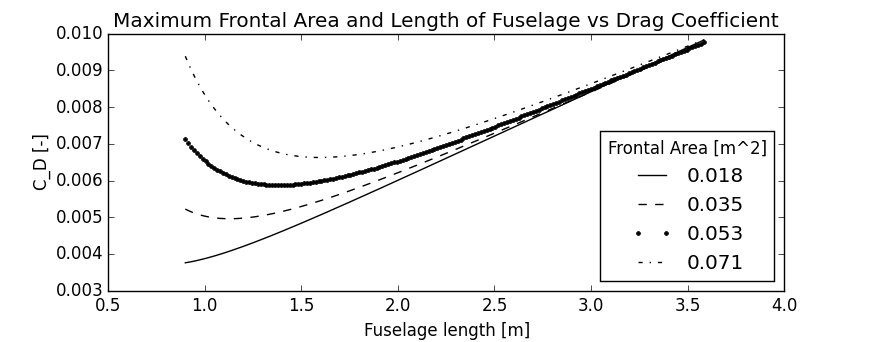
\includegraphics[width=0.8\textwidth]{Aerodynamics/Figures/fusdrag}
    \caption{Influence of Maximum Frontal Area and Fuselage Length on Drag Coefficient}
    \label{fig:fusdrag}
\end{figure}

Since the cross sectional area of the fuselage is mostly dictated by the payload bay and the structures department, the maximum frontal area is fixed at $0.053 m^{2}$. At this frontal area, the optimal fuselage length is 1.4 meters. The minimal length was limited to 1.7 meters by the structures department, nevertheless the final fuselage length was set to 1.8 meters. The reason for this was to have a less abrupt fuselage ending by elongating the empennage by 10 centimetres, in anticipation of a lower pressure drag. Although this contradicts the optimisation, it should be noted that the parametric equations assume that the fuselage cross sectional area gradually decreases towards the aft of the UAV, and this is not the case for the Hybrid UAV. To approximate this situation, the empennage is elongated, resulting in a $C_{D}$ of 0.0062 and a drag of 2.7 N at cruise velocities.

\nomenclature[B]{$C_{D}$}{Drag coefficient \nomunit{-}}

The results of the SimScale Workbench indicate a drag of 2.2 N during cruise. The validity of this result is discussed in \autoref{sub:vval}.

\subsection{Pylon}
\label{sec:aero_pylo}

\paragraph{Literature Study} The design of the pylon is performed in a similar fashion to the fuselage, with the goal to minimise the drag. Therefore the knowledge gained from the fuselage literature study is directly applicable to the pylon design. Furthermore, the same parametric equations can be used as for the fuselage \cite[73]{roskam}. The pylon-fuselage interference is considered significant enough to be included in the analysis, therefore the relevant parametric equations should also be used \cite[77]{roskam}.

\paragraph{Method} The parametric equations for the pylon were coded in the same manner as the one for the fuselage, with the addition of the pylon-fuselage interference equation. In this case, the two independent variables were the pylon length and the pylon diameter, and the output was the drag coefficient of the pylon. The results were plotted which made it possible to optimise the design for minimal drag.

Once the pylon shape was fixed, the CFD analysis was performed in order to gain more accurate drag values. This analysis was also carried out in the same manner as the main wing.

\paragraph{Results} The influence of the pylon diameter and length on the drag is shown in the plot in \autoref{fig:pyldrag}. It can be seen that the smaller the diameter, the smaller the drag coefficient. Furthermore, for each diameter there is an optimal pylon length resulting in a minimal drag coefficient.

\begin{figure}[H]
    \centering
    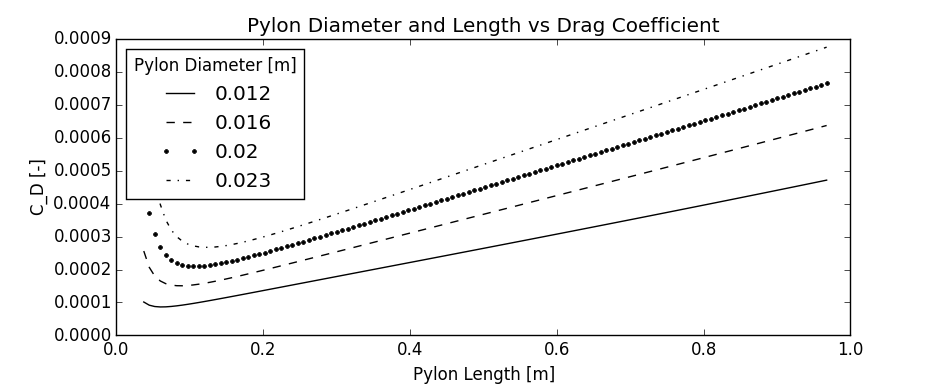
\includegraphics[width=0.8\textwidth]{Aerodynamics/Figures/pyldrag}
    \caption{Influence of Pylon Diameter and Length on Drag Coefficient}
    \label{fig:pyldrag}
\end{figure}

The minimal diameter is dictated by the structures department, therefore it is fixed at 2 cm. The corresponding optimal pylon length is 10.5 cm, yet the minimal possible length set by the stability \& control department is 90 cm. The result of the parametric analysis is a $C_{D}$ of 0.00072 and a drag of 0.317 N at cruise velocities.

The results of the SimScale Workbench indicate a drag of 0.248 N during cruise. The validity of this result is discussed in \autoref{sub:vval}.

\section{Verification \& Validation}
\label{sec:aero_vali}

In order to ensure that the 3D analyses were carried out correctly, the methods have to be verified, and the results validated. The verification of the XFLR5 tool is considered first. The validation of the wing, tail, fuselage, and pylon results is treated afterwards.

\subsection{XFLR5 Verification}

XFLR5 uses an inviscid linear-vorticity panel method to calculate the aerodynamic characteristics of airfoils \cite[1]{xfoil}. Therefore, in order to test whether this model produces accurate results within XFLR5, two verification methods are used. For convenience, the NACA 4417 airfoil will be used as an example.

\paragraph{Analytical} The first method consists of finding the $C_{l}-\alpha$ curve using the classical cambered thin airfoil theory \cite[348]{anderson}, where the lift coefficient is described by \autoref{eq:cl_anal}:

\begin{equation}
\label{eq:cl_anal}
    C_{l} = \pi \Big{(}2\alpha+\frac{2}{\pi}\int_{0}^{\pi}\frac{dz}{dx}\cos{\theta}d\theta-\frac{2}{\pi}\int_{0}^{\pi}\frac{dz}{dx}d\theta\Big{)}
\end{equation}
Here, $z$ describes the mean camber line geometry as a function of the chord position $\frac{x}{c}$. For the 4-digit NACA family, the derivative of the mean camber line geometry with respect to the chord position is given by \autoref{eq:naca_geo1} and \ref{eq:naca_geo2}\footnote{\url{http://airfoiltools.com/airfoil/naca4digit}, Accessed on 20-06-2017}:


\begin{equation}
\label{eq:naca_geo1}
    \frac{dz}{dx} = \frac{2m}{p^{2}}\big{(}\frac{p}{10}-\frac{x}{c}\big{)} \quad for \quad 0 \leq x \leq pc/10
\end{equation}
\begin{equation}
\label{eq:naca_geo2}
    \frac{dz}{dx} = \frac{m}{50(1-p/10)^{2}}\big{(}\frac{p}{10}-\frac{x}{c}\big{)} \quad for \quad pc/10 \leq x \leq c
\end{equation}
Here, the variables $m$ and $p$ are the first two digits of the NACA airfoil description (i.e. NACA mpXX). In order to be able to insert the above equations into \autoref{eq:cl_anal}, the variable change shown in \autoref{eq:varc} must take place:

\begin{equation}
\label{eq:varc}
    \frac{x}{c} = \frac{1}{2}(1-\cos{\theta})
\end{equation}
Solving the equation for the NACA 4417 airfoil yields \autoref{eq:analres}:

\begin{equation}
\label{eq:analres}
    C_{l} = 2\pi\alpha + 0.356
\end{equation}

\nomenclature[G]{$\alpha$}{Angle of attack \nomunit{deg}}
\nomenclature[G]{$\alpha$}{Angle of attack \nomunit{rad}}
\nomenclature[B]{$z$}{Mean camber line height\nomunit{-}}
\nomenclature[B]{$\frac{x}{c}$}{Position along airfoil chord\nomunit{-}}
\nomenclature[B]{$\frac{dz}{dx}$}{Mean camber line slope\nomunit{-}}
\nomenclature[G]{$\theta$}{Independent variable of the circular description of an airfoil geometry\nomunit{rad}}
\nomenclature[B]{$m$}{Airfoil maximum camber as a fraction of the chord multiplied by 100\nomunit{-}}
\nomenclature[B]{$p$}{Airfoil maximum camber position as a fraction of the chord multiplied by 10\nomunit{-}}
\nomenclature[B]{$c$}{Airfoil chord\nomunit{m}}

\paragraph{Numerical} The second method consists of finding the $C_{l}-\alpha$ curve using the vortex panel numerical method \cite[361]{anderson}, where the lift coefficient is found by dividing the airfoil into panels and solving for the vortex strength ($\Gamma$) at each panel using \autoref{eq:solve}.

\begin{equation}
\label{eq:solve}
    V_{\infty}\Big{(}\alpha - \frac{dz}{dx}\Big{)} + w_{induced} = 0
\end{equation}
Here, the induced velocity ($w_{induced}$) is given by \autoref{eq:indu} for an n-number of panels. Here $x_{cp}$ denotes the position of the control point, and $x_{\Gamma}$ denotes the position of the vortex, both as a fraction of the chord length.

\begin{equation}
\label{eq:indu}
    w_{induced} = \sum\limits_{i=1}^n \frac{-\Gamma_{i}}{2\pi(x_{cp,i}-x_{\Gamma,i})}
\end{equation}
For the purpose of this verification, the airfoil was divided into two equal panels, the vortices were placed at the quarter chord points of each panel, and the control points were placed at the three-quarters chord points of each panel. Solving for the NACA 4417 airfoil, the two panel vortex strengths are given by \autoref{eq:vortex}:

\begin{equation}
\label{eq:vortex}
    \Gamma_{1} = \frac{3\pi c V_{\infty}}{8}\Big{(}2\alpha + \frac{67}{720}\Big{)} \quad \Gamma_{2} = \frac{3\pi c V_{\infty}}{8}\Big{(}\frac{2\alpha}{3} + \frac{79}{720}\Big{)}
\end{equation}
Plugging the values for the vortex strengths into \autoref{eq:numecl} yields the $C_{l}-\alpha$ relationship.

\begin{equation}
\label{eq:numecl}
    C_{l} = \frac{2(\Gamma_{1} + \Gamma_{2})}{cV_{\infty}}
\end{equation}

From the comparison between the analytical, numerical, and the XFLR5 $C_{l}-\alpha$ curves seen in \autoref{fig:vercompa}, it can be said that XFLR5 produces accurate results in the linear region of the curve. Therefore the model used by XFLR5 can be considered to be verified.

\begin{figure}[H]
    \centering
    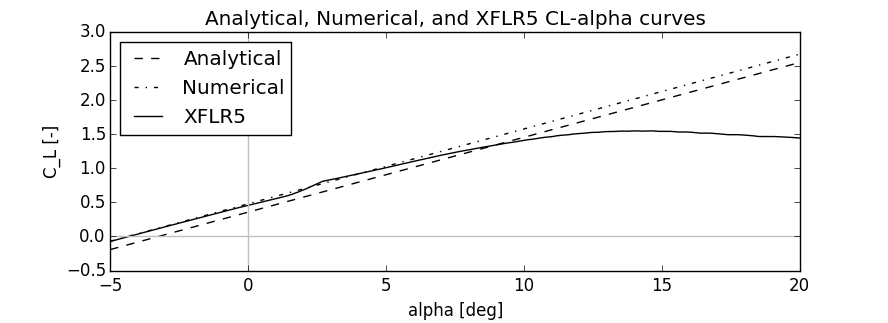
\includegraphics[width=0.8\textwidth]{Aerodynamics/Figures/vercomp}
    \caption{Comparison Between the Analytical, Numerical, and XFLR5 $C_{l}-\alpha$ Curves}
    \label{fig:vercompa}
\end{figure}

%- analytical thin airfoil theory
%- numerical panel method
%- summation of cl over span

%-verified by experience of other people

\nomenclature[B]{$V_{\infty}$}{Undisturbed airflow velocity\nomunit{m/s}}
\nomenclature[B]{$w_{induced}$}{Induced velocity\nomunit{m/s}}
\nomenclature[G]{$\Gamma$}{Vortex strength\nomunit{$m^{2}/s$}}
\nomenclature[B]{$x_{cp}$}{Position of the panel control point as a fraction of the airfoil chord\nomunit{-}}
\nomenclature[B]{$x_{\Gamma}$}{Position of the panel vortex as a fraction of the airfoil chord\nomunit{-}}
 
\subsection{Results Validation}
\label{sub:vval}

\paragraph{Wing} The validation of the wing results begins with the visual inspection of the spanwise lift distribution in order to ensure that it is elliptical (as intended). A comparison between the two is plotted and seen in \autoref{fig:wdist}. It can be seen that the lift distribution closely approximates an elliptical one, therefore this result is considered to be valid.

\begin{figure}[H]
    \centering
    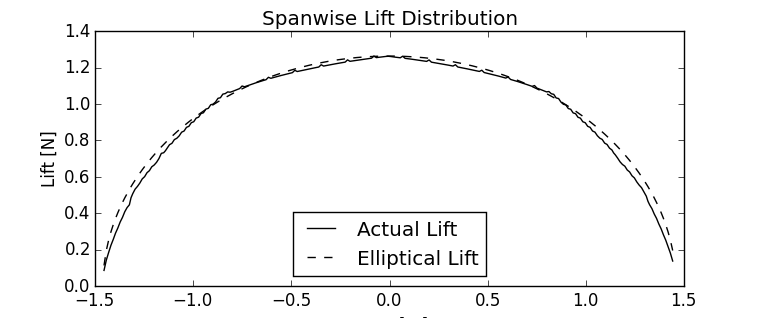
\includegraphics[width=0.8\textwidth]{Aerodynamics/Figures/wdist}
    \caption{Comparison of Actual and Elliptical Lift Distribution}
    \label{fig:wdist}
\end{figure}

The next step is to validate the lift and drag obtained from the SimScale Workbench tool. This is done by comparing the SimScale results to the XFLR5 ones. As seen in the 3D Wing Results in \autoref{sec:aero_wing}, the discrepancy is too large and thus this result is not considered valid. One possible reason for the discrepancy is an improper boundary condition implementation, yet due to resource constraints this claim was not proven. However, since XFLR5 tool was verified, its results are considered to be valid. Therefore the final lift and drag coefficients of the wing are 0.444 and 0.015 respectively.

\paragraph{Tail} The validation of the tail results consists of only a comparison between the SimScale Workbench and XFLR5 results. These forces (as seen in the 3D Tail Results in \autoref{sec:aero_tail}) are similar and in the same order of magnitude as the XFLR results, therefore it is assumed that the setup of the CFD was correct, and the tail lift and drag coefficient is updated to 0.213 and 0.0026 respectively.

\paragraph{Fuselage and Pylons} The validation of the fuselage and pylon results consists of a comparison between the SimScale Workbench and parametric results. 

As seen in the Results in \autoref{sec:aero_fuse}, the fuselage drag force obtained from the SimScale Workbench tool is similar and in the same order of magnitude as the parametric result, therefore it is assumed that the setup of the CFD (including the initial and boundary conditions) was correct and the results are considered valid. Hence, the fuselage drag coefficient is updated to 0.005.

The results in \autoref{sec:aero_pylo} show that the pylon drag force obtained from the SimScale Workbench tool is also similar and in the same order of magnitude as the parametric result, therefore it is assumed that the setup of the CFD was correct and the results are considered valid. Hence, the pylon drag coefficient is updated to 0.00056.
